\documentclass[12pt]{article}
\usepackage[utf8]{inputenc}

% Importing settings from setup.sty
\usepackage{setup}
\usepackage{booktabs}
\usepackage{multicol}
\usepackage{multirow}
\usepackage{glossaries}
% \makenoidxglossaries
% \newcommand{\thetahat}{\hat{\theta}}

\newacronym{bmi}{BMI}{Body Mass Index}


% \pagenumbering{roman}
\begin{document}

% Inserting title page
\import{./}{title}

\pagenumbering{gobble}
\tableofcontents
\listoffigures
\listoftables



\newgeometry{
  left=25mm,
  right=25mm,
  top=25mm,
  bottom=25mm}
\pagenumbering{arabic}
\section{Assignment 1}
\subsection{Exercise 1}
The code was completed in the Python file.

\subsection{Exercise 2}
\subsubsection{Question 1}
I was not familiar with the PyTorch library, so I had to perform some research in order to know how its methods/classes work.
I consulted several sources, including the following, which were useful in order to answer this question:
\begin{enumerate}
  \item \href{https://discuss.pytorch.org/t/how-sgd-works-in-pytorch/8060/2}{https://discuss.pytorch.org/t/how-sgd-works-in-pytorch/8060/2}
  \item \href{https://discuss.pytorch.org/t/performing-mini-batch-gradient-descent-or-stochastic-gradient-descent-on-a-mini-batch/21235}{https://discuss.pytorch.org/t/performing-mini-batch-gradient} \\
        \href{https://discuss.pytorch.org/t/performing-mini-batch-gradient-descent-or-stochastic-gradient-descent-on-a-mini-batch/21235}{-descent-or-stochastic-gradient-descent-on-a-mini-batch/21235}

  \item \href{https://pytorch.org/docs/stable/generated/torch.optim.SGD.html}{https://pytorch.org/docs/stable/generated/torch.optim.SGD.html}
\end{enumerate}
According to those sources, PyTorch's SGD actually computes a full-batch (vanilla) Gradient Descent, based on the data that is passed to it.
It is my understanding that in order to perform actual mini-batch (\ie where $1 < \text{batch size} < \text{number of observations}$), one simply needs to give subsets of the data a each iteration. \\
In our case, we use the full dataset in \texttt{outputs = net(inputs)}, which is why we perform full-batch GD, although we call the \texttt{optim.SGD} class.

\subsubsection{Question 2}
Figures \ref{fig: loss comparison 1-300}, \ref{fig: loss comparison 2-10-10} and \ref{fig: loss comparison 2-20-20} show a comparison between train and test cross entropy loss.
The leftmost diagrams have a linear scale for the vertical axis, while the rightmost diagrams have a logarithmic scale for the vertical axis.
Beware that the number of epochs varies significantly between figures.
Indeed, more pararmeters in the network implies longer training times per epoch, which in turn means that running for the same time both experiments results in different number of epochs. \\
\begin{figure}[ht]
  \centering
  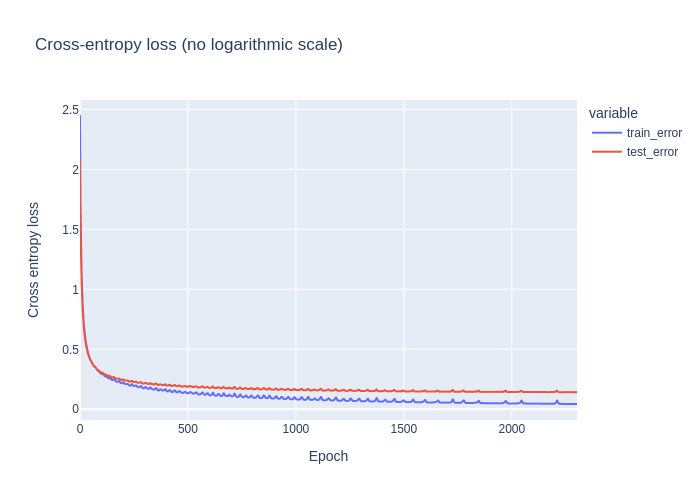
\includegraphics[width=0.49\textwidth]{images/cross-entropy-comparison-1-300.png}
  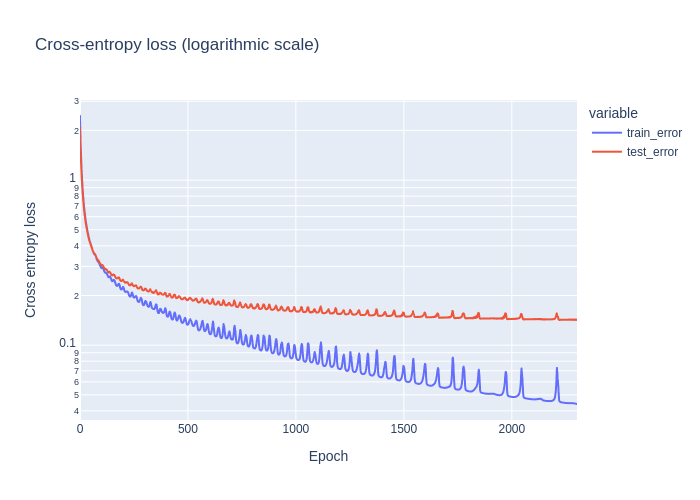
\includegraphics[width=0.49\textwidth]{images/cross-entropy-comparison-1-300-log.png}
  \caption{Cross entropy loss, train vs test ($300$ fully-connected)}
  \label{fig: loss comparison 1-300}
\end{figure}
\begin{figure}[ht]
  \centering
  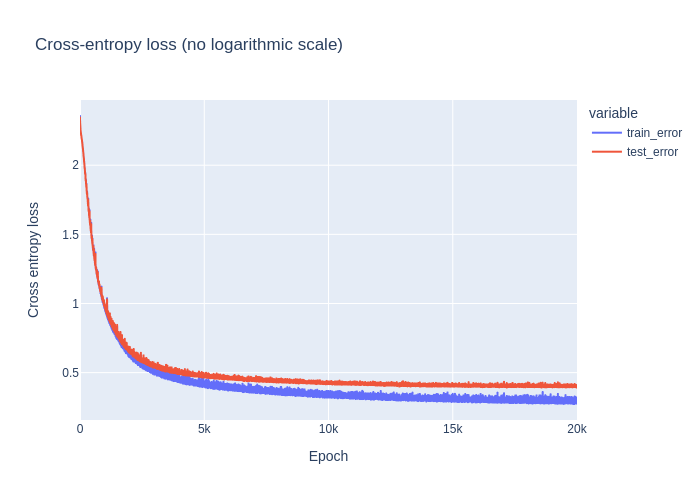
\includegraphics[width=0.49\textwidth]{images/cross-entropy-comparison-2-10-10.png}
  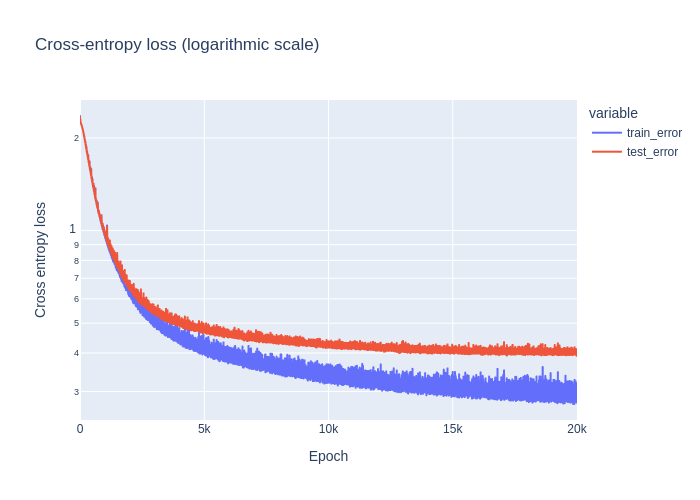
\includegraphics[width=0.49\textwidth]{images/cross-entropy-comparison-2-10-10-log.png}
  \caption{Cross entropy loss, train vs test ($10-10$ fully-connected)}
  \label{fig: loss comparison 2-10-10}
\end{figure}
\begin{figure}[ht]
  \centering
  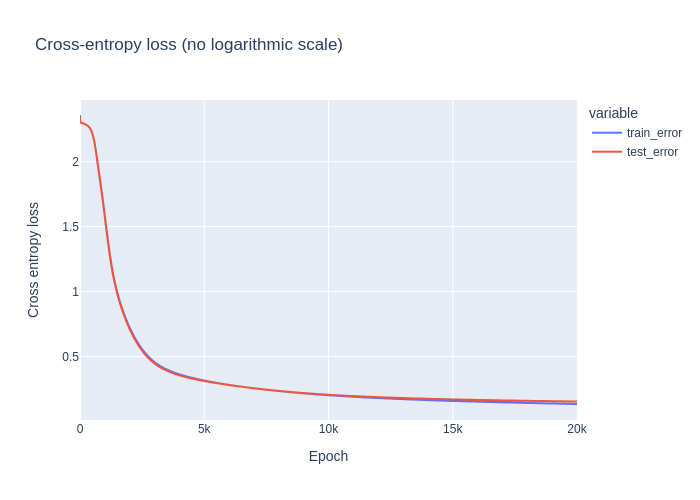
\includegraphics[width=0.49\textwidth]{images/cross-entropy-comparison-2-20-20.png}
  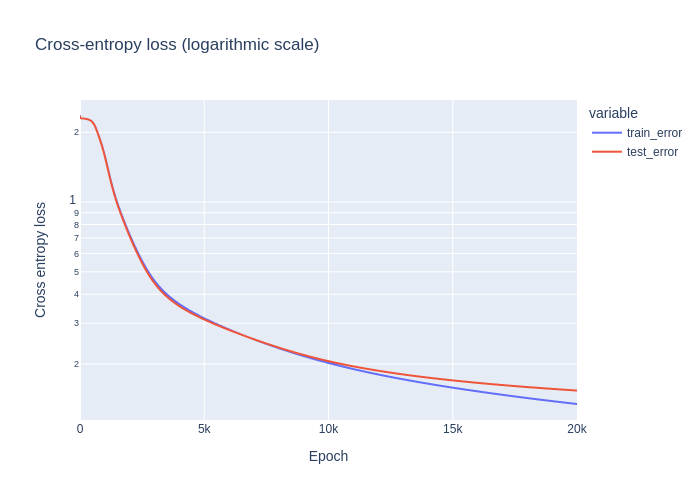
\includegraphics[width=0.49\textwidth]{images/cross-entropy-comparison-2-20-20-log.png}
  \caption{Cross entropy loss, train vs test ($20-20$ fully-connected)}
  \label{fig: loss comparison 2-20-20}
\end{figure}
We see that in both experiments the train error keeps decreasing, while the test error stays constant.
This means that our network is overfitting and there is no need to continue the experiment further.
One way to prevent wasting time training when the network isn't making actual progress is to print the loss, or even to plot the loss curves, every couple iterations.
We estimate however that the over-fitting phenomenon isn't too extreme in our case.

\subsubsection{Question 3}
Let $\beta: \N^{l+1} \to \N$ denote the number of parameters in a fully connected neural network. Then $\beta$ is given by:
\begin{equation}
  \beta(h_0, \ldots, h_l) := \sum_{i=1}^{l} (h_{i-1} * h_{i}) + h_i
\end{equation}
Indeed, the multiplication term ``$h_{i-1} * h_{i}$'' accounts for the weights by counting the connections from a layer to the next.
The last term ``$h_i$'' is responsible for counting the biases on each of the hidden layers, as well as the output layer. \\
We compute $\beta$ for a few network architectures we used, with $h_0 = 28 * 28 = 784$ in all cases, since this is the size of the input:
\begin{align*}
  \beta(784, 10, 10, 10)
   & = (784 * 10 + 10) + (10 * 10 + 10) + (10 * 10 + 10) \\
   & = 7850 + 110 + 110                                  \\
   & = 8070                                              \\
\end{align*}
\begin{align*}
  \beta(784, 20, 20, 10)
   & = (784 * 20 + 20) + (20 * 20 + 20) + (20 * 10 + 10) \\
   & = 15700 + 420 + 210                                 \\
   & = 16330                                             \\
\end{align*}
\begin{align*}
  \beta(784, 300, 10)
   & = (784 * 300 + 300) + (300 * 10 + 10) \\
   & = 235500 + 3010                       \\
   & = 238510                              \\
\end{align*}
However, we know that not all parameters are created equal.
Indeed, adding more layers includes non-linearities in the network.
Increasing the number of layers is useful because it ``bends" the space in which the data lives, which allows to find more patterns.
On the other hand, adding layers causes other issues, namely the vanishing gradient problem: as the gradient goes through multiple activation functions, it shrinks until making close to no update in the weight.
The argument for less layers is also strengthened by Cybenko's \textit{Universal approximation theorem} (1989), which proves that a unique hidden layer is sufficient to approximate any \textit{reasonable} function with arbitrary precision.
However, it may require the hidden layer to be of exponential size with respect to the desired precision. \\
The bottom line to this reflexion is as follows: increasing the size of the layers is good because the network can learn more, however there are risks of overfitting.
Increasing the number of layers is also an option, but it can cause overfitting and gradients may vanish. \\
Most certainly some trial and error is required, with close baby-sitting of training and validation errors in order to adapt the architecture.


\subsubsection{Question 4}
In PyTorch, with NLLLoss meaning Negative Log-Likelihood Loss:
\begin{equation}
  CrossEntropyLoss = SoftMax \circ NLLLoss
\end{equation}
The $NLLLoss$ part isn't too much of interest as it simply outputs the most likely class. The SoftMax function however is more interesting. Indeed, it acts as a normalized exponential and therefore outputs probabilities. This is not true with quadratic loss that can output any non-negative number.


\subsubsection{Question 5}
Using a single output means that the network give us one definitive answer and we have no idea of how certain it is.
One hot encoding on the other hand provides probabilities of how sure it is when it makes predictions.
This is useful because a network should be penalized equally for different degrees of certainty.
Ideally, we want the network to be certain of its prediction and the prediction to be right.
If the network is certain of a wrong prediction, we should penalize it a lot.
We would prefer a network that makes a wrong prediction but is unsure.
This latter network would take less weights adjustments in order to make the prediction right.

\subsubsection{Question 6}
For this question, we will keep the architecture of a single 300-neurons hidden layer and we will monitor the loss with various learning rates. \\
Let us call the learning rate $\eta$. We already tested the case $\eta = 0.1$ in figure \ref{fig: loss comparison 1-300}.
Table \ref{table: figures per learning rate} gives a summary of associated figures for various values of $\eta$.
\begin{table}[h]
  \centering
  \begin{tabular}{c|c}
    Learning rate ($\eta$) & Figure number                             \\ \hline
    0.001                  & \ref{fig: learning rate comparison 0.001} \\
    0.1                    & \ref{fig: loss comparison 1-300}          \\
    0.3                    & \ref{fig: learning rate comparison 0.3}   \\
    0.5                    & \ref{fig: learning rate comparison 0.5}   \\
    0.7                    & \ref{fig: learning rate comparison 0.7}   \\
    0.9                    & \ref{fig: learning rate comparison 0.9}   \\
    1.2                    & \ref{fig: learning rate comparison 1.2}   \\
    2                      & \ref{fig: learning rate comparison 2}     \\
    5                      & \ref{fig: learning rate comparison 5}     \\
    8                      & \ref{fig: learning rate comparison 8}     \\
  \end{tabular}
  \caption{Figure number per learning rate}
  \label{table: figures per learning rate}
\end{table}
The figures in table \ref{table: figures per learning rate} are located in appendix \ref{appendix: varying learning rates}.

\paragraph{Result analysis}
It is my understanding that learning rates are often of order $\eta = 10^{-k}$ for $k = 1, \ldots, 4$. In this case however, this is not what I found at all. Indeed, we see that learning rates $\eta \in \{ 0.001, 0.1, 0.3, 0.5, 0.7, 0.9, 1.2, 2 \}$ converge nicely even though converging rates vary. For instance, $\eta = 2$ converges faster than lower values. One may be tempted to increase $\eta$ even further. On the other hand, we see that larger learning rates such as $\eta \in \{ 5, 8 \}$ result in instabilities, but $\eta = 5$ still reaches good (low) values of cross entropy loss. \\
We didn't try every possible value of $\eta$ but it seems that somewhere between $\eta = 2$ and $\eta = 5$ could be a good candidate. Smaller values do indeed converge, but take many epochs (\ie long times), while larger values tend to ``overshoot'' over minima from times to times, resulting in irregularities in their gradient descent procedure. \\
One thing worth noting is that we tested all learning rates over 2000 epochs. Such a number of epochs wasn't too long on my machine but also wasn't ridiculously low, which allows to reach decent loss values. We must note that we are probably putting low learning rates at a disadvantage because they most certainly converge as expected, but also take longer to do so (steps in the right direction, but small steps).


\subsubsection{Question 7}
The layer described in question 3 is a 300 neurons (single) hidden layer. As a result, only 2 gradients are computed (input to hidden and hidden to output). The vanishing gradient problem tends to occur on networks with more hidden layers. In such cases, gradients have to go through activation functions several times. Doing so squishes them between 0 and 1 (for many activation functions, \eg Sigmoidal, SoftMax) multiple times. As a result, gradients end up going to 0 and eventually make no update to the weights anymore. \\
Several solutions can be implemented in order to solve the vanishing gradient problem. Here are some of them:
\begin{itemize}
  \item The simplest, most radical way to solve the vanishing gradient problem is to remove hidden layers. This removes some of the activation functions that are applied to the gradient.
  \item On complex problems however, removing hidden layers may not be an option because there is may be more information to discover in the data. In such cases, one may use ReLU as an activation function, where ReLU is defined as follows:
        $$
          ReLU(x) := \max (0, x)
        $$
        ReLU is faster than many other activation functions because it has less computations to make (computing exponentials, summing, dividing, \ldots). ReLU leaves positive gradients unchanged and sets negative ones to 0, in particular it doesn't squish gradients. This solves the vanishing gradient problem in most cases. \\
        Although ReLU often solves the vanishing gradient problem, it also comes with its downsides, namely making gradients explode.
  \item Another way to solve the vanishing gradient problem is to use residuals. Indeed, by randomly setting some weights in the network to 0, the network ``learns to use alternative routes'' (grossely speaking). This also tends to fix the vanishing gradient problem.
\end{itemize}



\section{Assignment 2}
I will start fresh for assignment 2 and reimplement some of the functions.

\subsection{Exercise 1}
Please allow us to give an overall feeling from the experiments I have performed, rather than reporting for each learning rate, for each batch size the result after a given number of epochs. \\
From the experiments conducted, we notice a few things. We will explain each of them.
\paragraph{Epochs take much longer as the batch size decreases}
This makes sense. As the batch size decreases, we have to go over more batches to complete one epoch. For each of these batches, we must compute the loss, compute the gradient and update the weights. As a result, there are more updates per epoch, which makes each epoch longer. This doesn't really matter though because instead of looking at the time per epoch, a more interesting metric would be the time per update. Although the time per epoch increases, there are actually $len(X\_train) / batch\_size$ updates per epoch, and each of these updates is faster than if the network had had to compute the gradients over the whole dataset.
\paragraph{High learning rates are not acceptable anymore}
This also makes sense. Consider the full-batch case (previously). Since the gradient was computed over the whole dataset, this was a (very long, but) very carefully chosen descent direction. As a result, it was acceptable to make a big step. In the minibatch setting however, the steps are way faster, but a bit more imprecise. For this reason, it is not wise anymore to take large steps anymore. Nevertheless, this option is still very interesting because we can take ``mostly correct'' steps very fast and make fast progress towards the minimum.
\paragraph{Minibatch is still the best method overall}
As mentioned previously, epochs do take longer and steps sizes must be reduced. We showed however that it doesn't matter because we make much more frequent updates, which are ``mostly in the right direction''. For this reason and according to our experiments, minibatch converges much faster than full batch. After only a couple epochs, we are already in a better place than after hundreds of epochs in the full batch case, which shows very interesting results in favor of mini batch.

\subsection{Exercise 2}
In the case where all parameters are set to 0, the network doesn't learn anything. After performing some searches, this is called the symmetry break. I will try to display my understanding without copy-pasting my sources (\href{https://stats.stackexchange.com/questions/45087/why-doesnt-backpropagation-work-when-you-initialize-the-weights-the-same-value}{1}, \href{https://stackoverflow.com/questions/20027598/why-should-weights-of-neural-networks-be-initialized-to-random-numbers}{2}). \\
When going from one layer to the next, what is applied is basically a given number of dot products. Let us consider the case of going from the input layer $I$ (size 784) to the first hidden layer $H_1$ (size 300). Let us disregard the bias here because the explanation is the same, but it brings confusion into the dimensions. Then this transition is done by multiplying the input matrix of size $(\text{n\_samples} \times 784)$ by a weight matrix $W_1$ of size $(784 \times 300)$. This gives a hidden layer of size $(\text{n\_samples} \times 300)$. The matrix that has all weights 0 in this case is $W_1$. If $W_1 = 0 \in \mathcal{M}_{(784 \times 300)}$, then each input vector is put through a dot product with a vector of $0$'s to give the corresponding entry of the hidden layer. As a result, all values of the hidden layer are equal (in this case, equal to 0). Then they all go through the activation function and are propagated through the rest of the network. For gradient descent to ``work'' however, the hidden layer should not contain all same entries. If each unit in the hidden layer gets the same signal, it will not propagate varied, useful information through the network, but only limited, redundant information.


\subsection{Exercise 3}
\subsubsection{Question 1}
% stubborn network

\subsubsection{Question 2}
\subsubsection{Question 3}
\subsection{Exercise 4}

\newpage
\appendix
\section{Varying learning rates}
\label{appendix: varying learning rates}
\begin{figure}[ht]
  \centering
  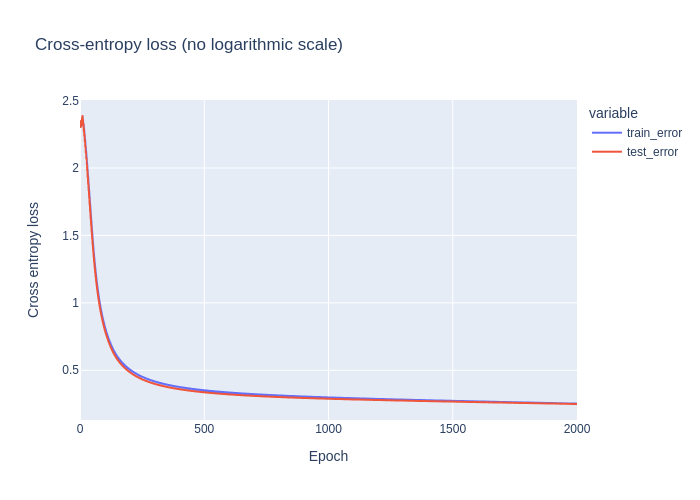
\includegraphics[width=0.49\textwidth]{images/cross-entropy-comparison-1-300-lr0.001.png}
  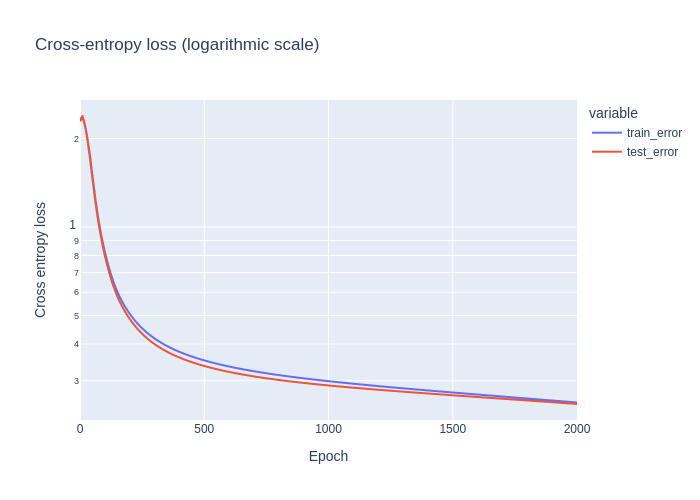
\includegraphics[width=0.49\textwidth]{images/cross-entropy-comparison-1-300-lr0.001-log.png}
  \caption{Cross entropy loss, train vs test ($300$ fully-connected), $\eta = 0.001$}
  \label{fig: learning rate comparison 0.001}
\end{figure}
\begin{figure}[ht]
  \centering
  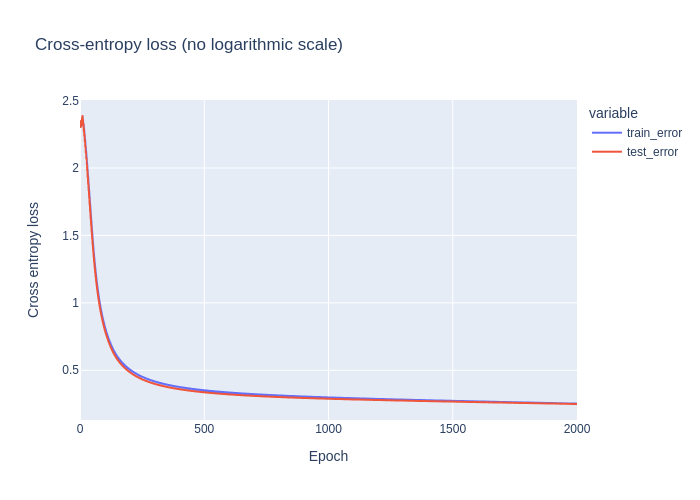
\includegraphics[width=0.49\textwidth]{images/cross-entropy-comparison-1-300-lr0.3.png}
  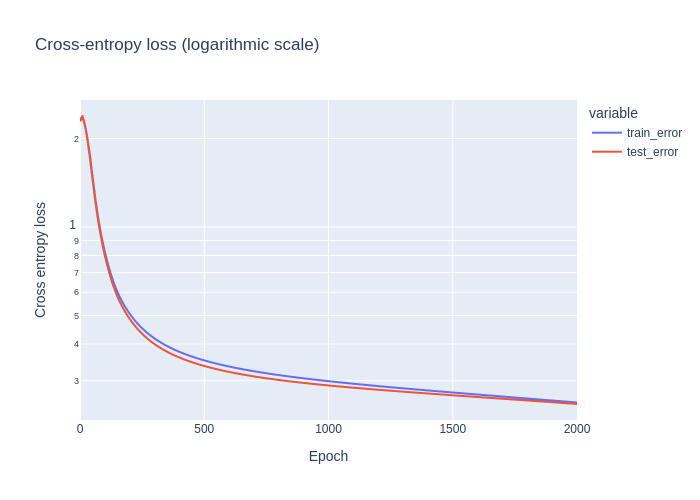
\includegraphics[width=0.49\textwidth]{images/cross-entropy-comparison-1-300-lr0.3-log.png}
  \caption{Cross entropy loss, train vs test ($300$ fully-connected), $\eta = 0.3$}
  \label{fig: learning rate comparison 0.3}
\end{figure}
\begin{figure}[ht]
  \centering
  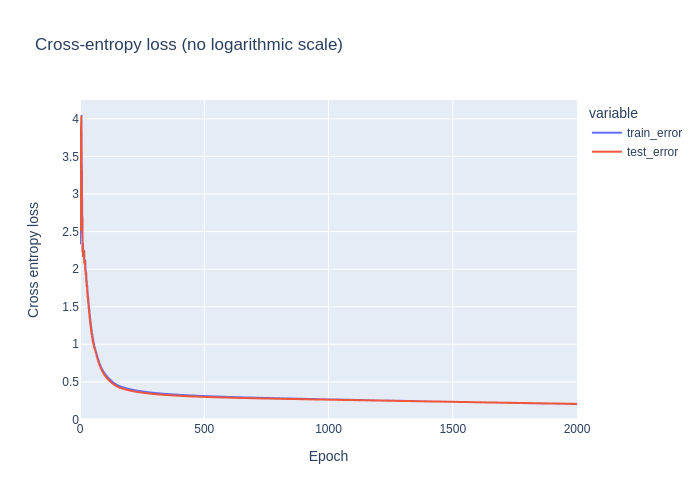
\includegraphics[width=0.49\textwidth]{images/cross-entropy-comparison-1-300-lr0.5.png}
  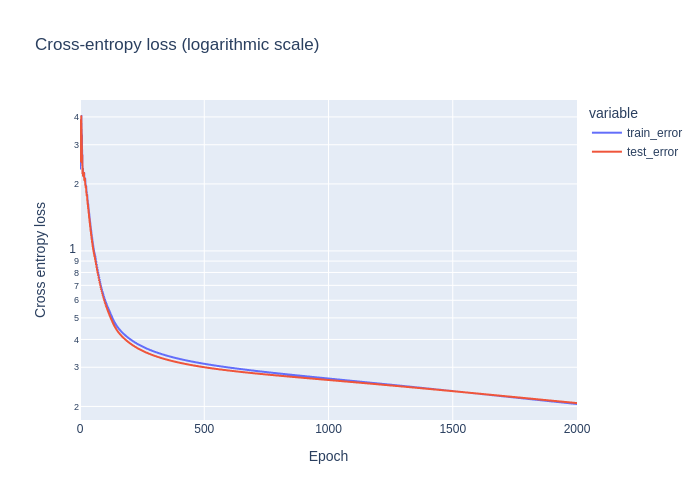
\includegraphics[width=0.49\textwidth]{images/cross-entropy-comparison-1-300-lr0.5-log.png}
  \caption{Cross entropy loss, train vs test ($300$ fully-connected), $\eta = 0.5$}
  \label{fig: learning rate comparison 0.5}
\end{figure}
\begin{figure}[ht]
  \centering
  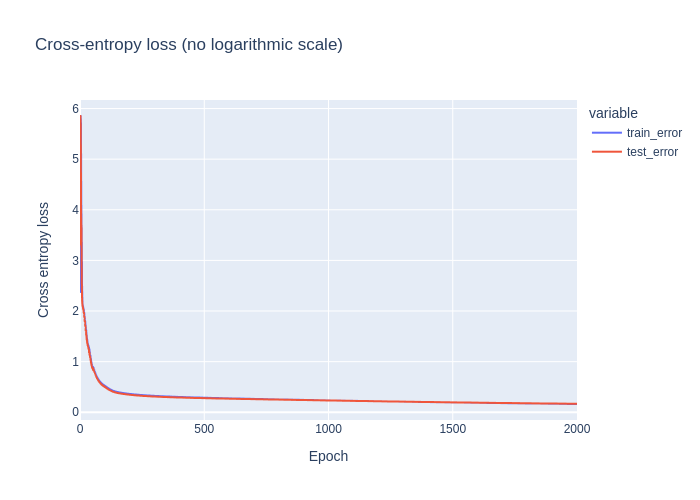
\includegraphics[width=0.49\textwidth]{images/cross-entropy-comparison-1-300-lr0.7.png}
  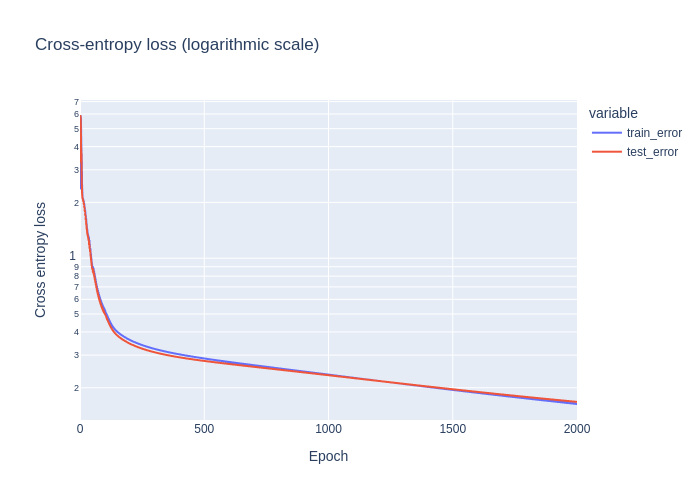
\includegraphics[width=0.49\textwidth]{images/cross-entropy-comparison-1-300-lr0.7-log.png}
  \caption{Cross entropy loss, train vs test ($300$ fully-connected), $\eta = 0.7$}
  \label{fig: learning rate comparison 0.7}
\end{figure}
\begin{figure}[ht]
  \centering
  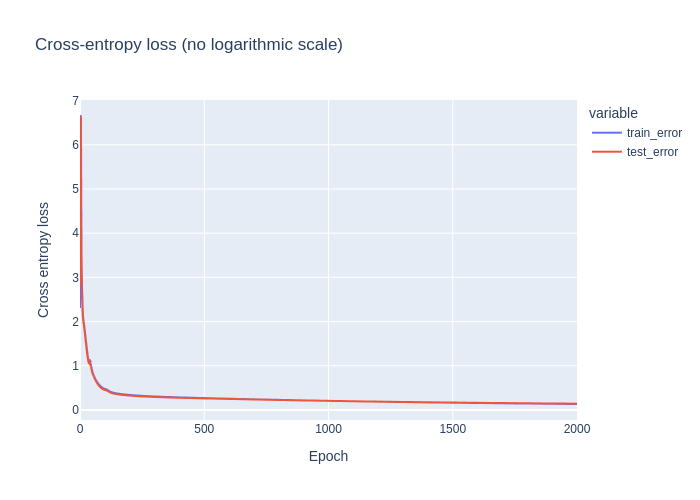
\includegraphics[width=0.49\textwidth]{images/cross-entropy-comparison-1-300-lr0.9.png}
  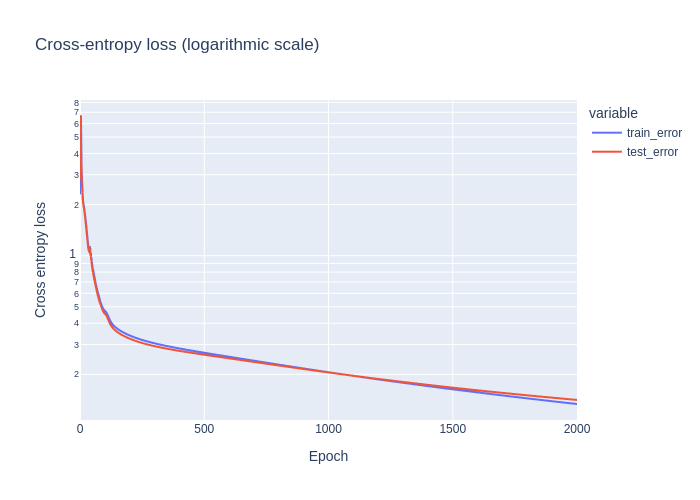
\includegraphics[width=0.49\textwidth]{images/cross-entropy-comparison-1-300-lr0.9-log.png}
  \caption{Cross entropy loss, train vs test ($300$ fully-connected), $\eta = 0.9$}
  \label{fig: learning rate comparison 0.9}
\end{figure}
\begin{figure}[ht]
  \centering
  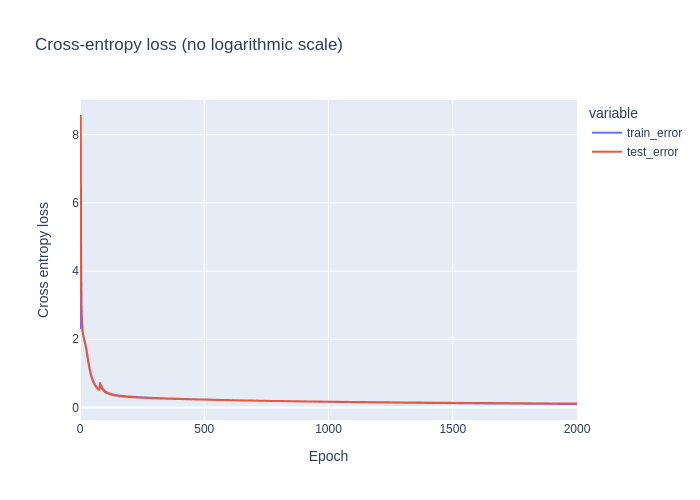
\includegraphics[width=0.49\textwidth]{images/cross-entropy-comparison-1-300-lr1.2.png}
  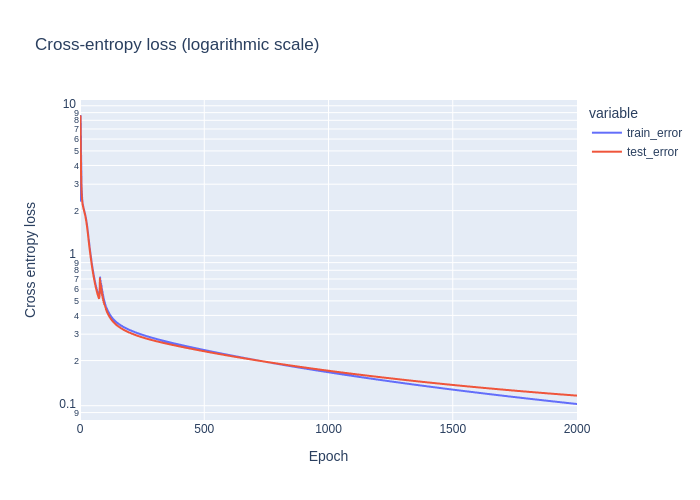
\includegraphics[width=0.49\textwidth]{images/cross-entropy-comparison-1-300-lr1.2-log.png}
  \caption{Cross entropy loss, train vs test ($300$ fully-connected), $\eta = 1.2$}
  \label{fig: learning rate comparison 1.2}
\end{figure}
\begin{figure}[ht]
  \centering
  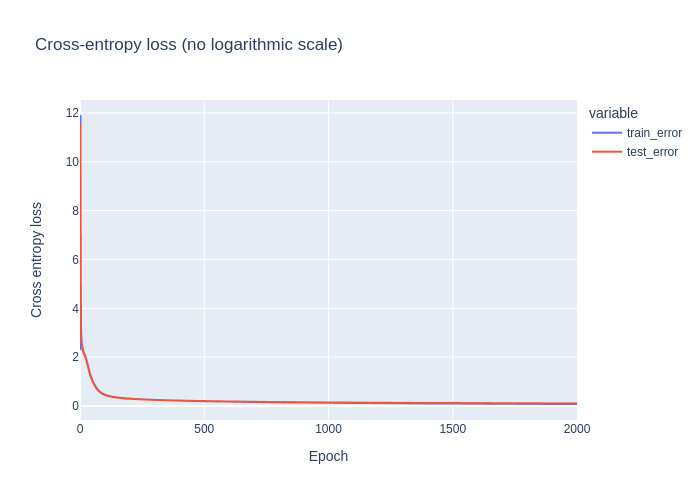
\includegraphics[width=0.49\textwidth]{images/cross-entropy-comparison-1-300-lr2.png}
  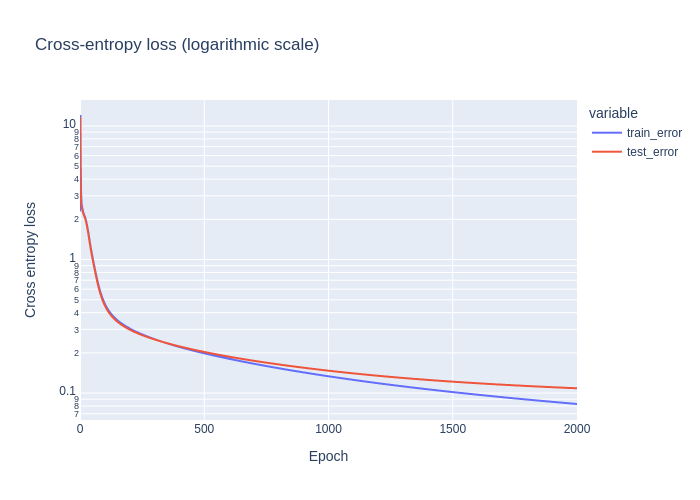
\includegraphics[width=0.49\textwidth]{images/cross-entropy-comparison-1-300-lr2-log.png}
  \caption{Cross entropy loss, train vs test ($300$ fully-connected), $\eta = 2$}
  \label{fig: learning rate comparison 2}
\end{figure}
\begin{figure}[ht]
  \centering
  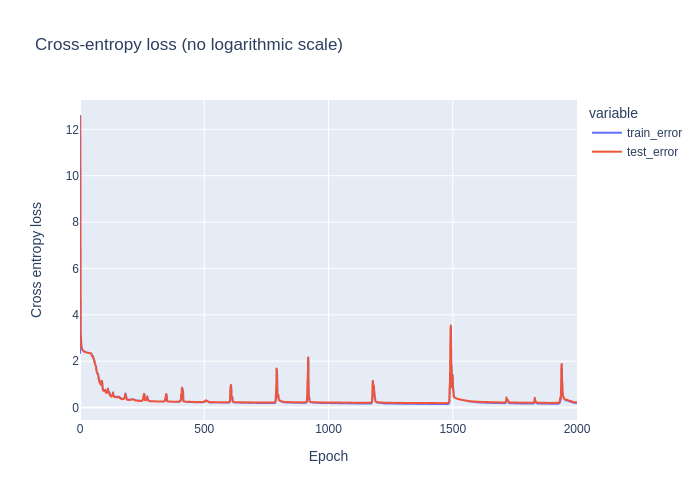
\includegraphics[width=0.49\textwidth]{images/cross-entropy-comparison-1-300-lr5.png}
  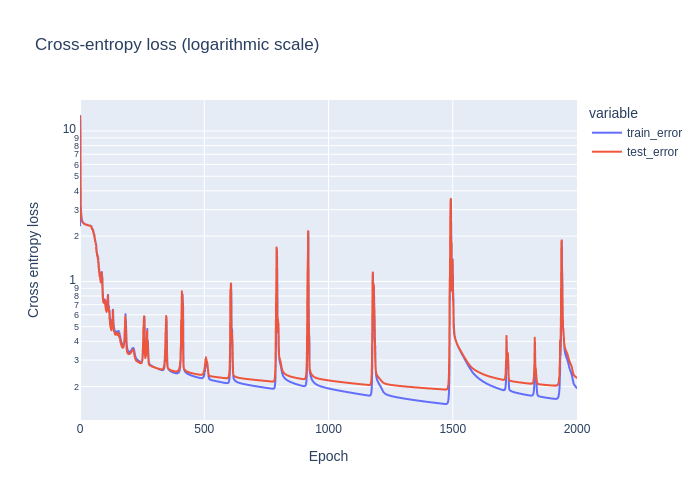
\includegraphics[width=0.49\textwidth]{images/cross-entropy-comparison-1-300-lr5-log.png}
  \caption{Cross entropy loss, train vs test ($300$ fully-connected), $\eta = 5$}
  \label{fig: learning rate comparison 5}
\end{figure}
\begin{figure}[ht]
  \centering
  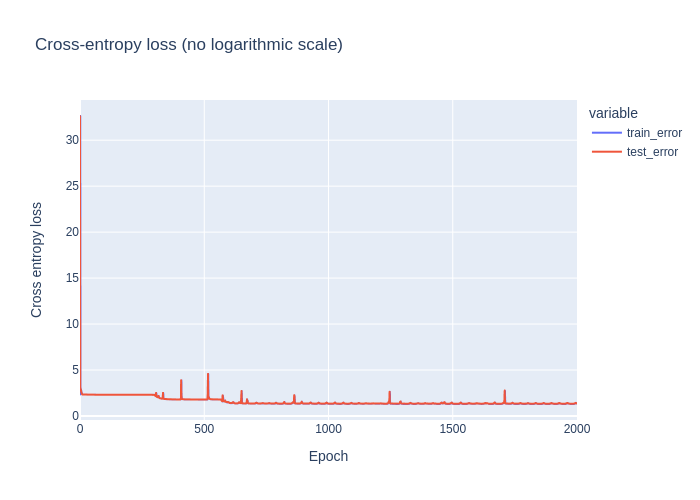
\includegraphics[width=0.49\textwidth]{images/cross-entropy-comparison-1-300-lr8.png}
  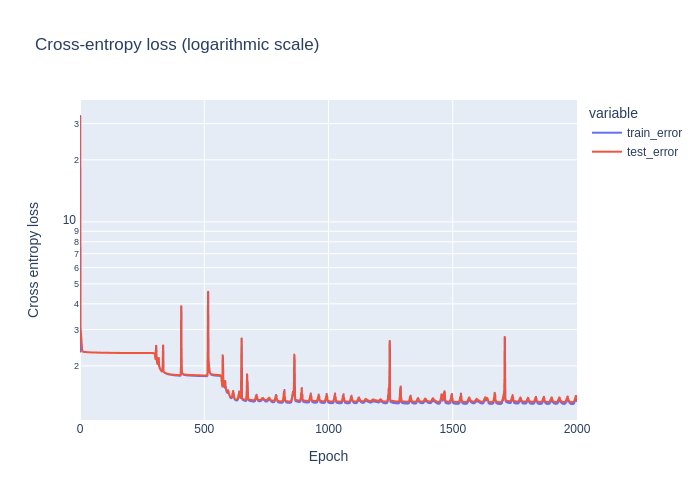
\includegraphics[width=0.49\textwidth]{images/cross-entropy-comparison-1-300-lr8-log.png}
  \caption{Cross entropy loss, train vs test ($300$ fully-connected), $\eta = 8$}
  \label{fig: learning rate comparison 8}
\end{figure}






\end{document}